\documentclass[11pt,letterpaper]{article}
\usepackage[utf8]{inputenc}
\usepackage{amsmath}
\usepackage{amsfonts}
\usepackage{amssymb}
\usepackage{geometry}
\usepackage{hyperref}
\usepackage{xcolor}
\usepackage{booktabs}
\usepackage{wrapfig}
\usepackage{caption}

% Brand Typography / Color configuration
\definecolor{mpdark}{HTML}{0F172A}
\definecolor{mpblue}{HTML}{3B82F6}
\definecolor{mpgreen}{HTML}{10B981}
\definecolor{mpred}{HTML}{EF4444}
\definecolor{mpblack}{HTML}{000000}

\usepackage{float} 
\usepackage{graphicx}
\graphicspath{{visual-assets/}} % Looks in the relative images folder

% Clean, modern margins
\geometry{margin=1in}

\hypersetup{
    colorlinks=true,
    linkcolor=mpblue,
    urlcolor=mpblue
}

\title{\textbf{\color{mpdark}Money Plot Labs Technical Whitepaper \\ The Pure Math of Financial Freedom}}
\author{\textbf{Harrison Hsueh} \\ \textit{Founder, Money Plot Labs}}
\date{May 2026}

\begin{document}

\maketitle

\begin{abstract}
This whitepaper derives the explicit, closed-form analytical solution for a fixed-horizon retirement timeline. By presenting a simple linear model first, we establish a transparent baseline using middle-school algebra. We then expand this model into exponential growth curves by mapping the exact continuous boundaries between an asset accumulation phase and an annuity-due depletion phase. This isolates the exact number of required working years ($w$) as a function of savings rate, spending targets, initial capital, investment growth, and desired legacy floors.
\end{abstract}

\section{Introduction \& Variables}
Standard personal finance paradigms rely on fragile rules of thumb. To achieve absolute mathematical certainty, we model an individual's financial lifecycle across a strictly bounded timeline from a starting age ($T_{\text{start}}$) to a maximum life expectancy ($T_{\text{end}}$). We define the total planning horizon as:
\begin{equation}
H = T_{\text{end}} - T_{\text{start}}
\end{equation}

Within this horizon $H$, an individual works for $w$ consecutive years and spends the remaining $f$ years in full retirement, such that:
\begin{equation}
H = w + f
\end{equation}

\subsection{Parameter Definitions}
\begin{itemize}
    \item $A_0$: Initial Net Worth / Starting Balance (\$)
    \item $c$: Annual Cash Savings Flow during working years (\$)
    \item $b$: Annual Retirement Budget Consumption (\$)
    \item $L$: Desired Capital Legacy Floor / Inheritance Remaining at Death (\$)
    \item $r$: Real Growth Rate adjusted for inflation
    \item $w$: Accumulation Phase duration (Working Years)
    \item $f$: Depletion Phase duration (Retirement Years)
\end{itemize}

---

\section{The Linear Baseline Case ($r = 0\%$)}
Before introducing the compounding curves of financial markets, we establish intuitive baselines by assuming real asset growth perfectly tracks inflation ($r = 0\%$). In this environment, wealth accumulates and depletes along perfectly straight lines, making it easy to isolate how system parameters structurally shift timeline horizons.

\subsection{Case 1: The Idealized Zero-Baseline Framework ($A_0 = 0, L = 0$)}
\begin{wrapfigure}{r}{0.5\textwidth} % {r} for left, {0.5\textwidth} for half width
    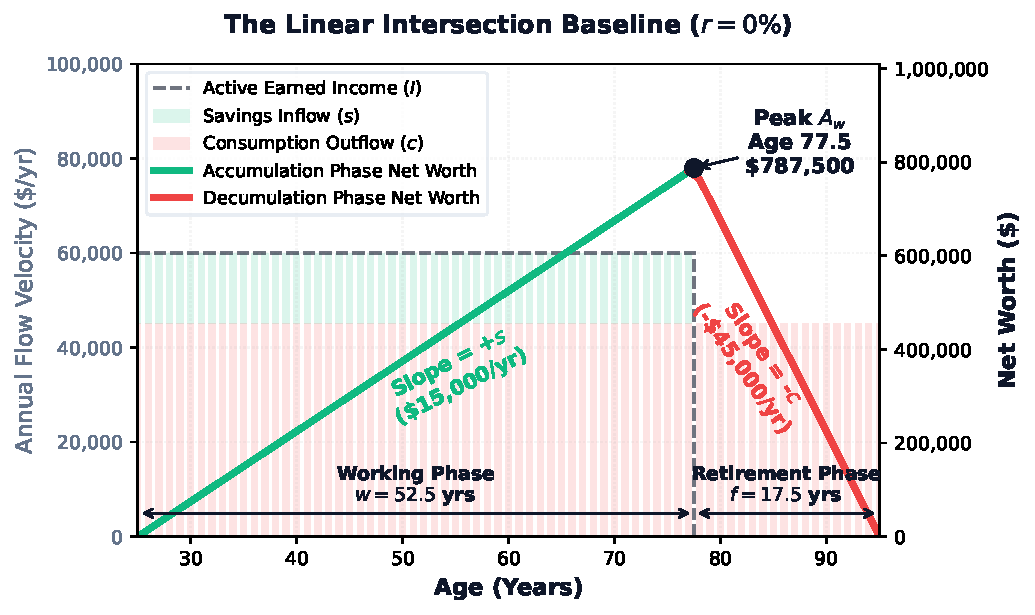
\includegraphics[width=\linewidth]{linear_plot.pdf}
    \captionsetup{textfont=small}
    \caption{The straight-line boundary crossover mapping where $r =0\%$. Assets accumulate smoothly via \textcolor{mpgreen}{labor} and deplete symmetrically via \textcolor{mpred}{consumption} until hitting the legacy boundary.}
\end{wrapfigure}
\vspace{2em}
We begin with a simplified world containing a zero starting balance ($A_0 = 0$) and no terminal inheritance target ($L = 0$). 

During the working phase, assets grow linearly via cash savings flow $c$ injected at the end of each period for $w$ years:
\begin{equation}
\text{Peak Assets Case 1} = c \cdot w
\end{equation}

Upon entering retirement, accumulation stops depletion begins draining our peak nest egg by a flat annual budget block $b$ for the remaining $f$ retirement years:
\begin{equation}
\text{Peak Assets Required Case 1} = b \cdot f
\end{equation}

To locate the precise intersection boundary where working ends and retirement begins, we enforce our system constraint where the peak accumulated capital must exactly equal the total retirement drawdown:
\begin{equation}
c \cdot w = b \cdot f
\end{equation}

Substituting our timeline identity $f = H - w$ allows us to solve for $w$:
\begin{equation}
c \cdot w = b \cdot (H - w)
\end{equation}

Grouping terms containing our target variable $w$ onto the left-hand side and factoring yields:
\begin{equation}
w(c + b) = b \cdot H
\end{equation}

Dividing through isolates our fundamental idealized baseline relationship:
\begin{equation}
w = \frac{b \cdot H}{c + b}
\end{equation}
In the example in Figure 1, $b = \$50,000\text{/year}$, $c = \$10,000\text{/year}$, \\
$T_{start} = \text{20 years}$, $T_{end} = \text{95 years}$.
\begin{align*}
    w &= \frac{\$50,000 \cdot 75 \text{ years}}{\$50,000 + \$10,000}\\
    w &= 62.5 \text{ years}
\end{align*}

\subsection{Case 2: The Parameterized Linear Solution with Boundary Modifiers ($A_0 \neq 0, L \neq 0$)}
We now expand our straight-line environment to account for real-world initial endowments and estate conservation goals. We reintroduce the asset head-start parameter ($A_0$) and the designated capital legacy floor ($L$). 

Incorporating these conditions alters our primary boundary accumulation and depletion states:
\begin{equation}
\text{Peak Assets Case 2} = A_0 + c \cdot w
\end{equation}
\begin{equation}
\text{Peak Assets Required Case 2} = L + b \cdot f
\end{equation}

Setting our parameterized accumulation trajectory equal to the absolute terminal requirement forces the system boundary equation:
\begin{equation}
A_0 + c \cdot w = L + b \cdot f
\end{equation}

Substituting our timeline identity $f=H-w$ and isolating our targeted timeline variables onto the left-hand side of the identity yields:
\begin{equation}
c \cdot w + b \cdot w = b \cdot H + L - A_0
\end{equation}

Factoring out $w$ collects our parameters into clean operational dimensions:
\begin{equation}
w(c + b) = b \cdot H + L - A_0
\end{equation}

Dividing through by our total structural velocity $(c + b)$ delivers the complete \textbf{Parameterized Linear Equation}:
\begin{equation}
w = \frac{b \cdot H + L - A_0}{c + b}
\end{equation}

This intermediate step clearly demonstrates the pure algebraic translation of our boundary mechanics: an initial balance ($A_0$) directly subtracts from required working years, while a desired legacy floor ($L$) extends the required labor timeline.

---

\section{Phase 1: The Exponential Accumulation Engine}
When we introduce real market investment returns ($r > 0\%$), our straight lines transform into curves. During the working phase ($w$), net worth grows via compound interest on the initial principal while absorbing an ordinary annuity flow of annual savings $c$ injected at the end of each period. The net worth at the exact boundary of retirement ($A_w$) is defined by:
\begin{equation}
{\color{mpgreen} A_w} = A_0(1+r)^w + c \cdot \frac{(1+r)^w - 1}{r}
\end{equation}

\subsection{Step-by-Step Inductive Derivation of $A_w$}
To understand the structural origin of the accumulation equation, we trace the boundary state changes sequentially at the close of each annual compounding cycle:
\begin{align*}
    A_1 &= A_0(1+r) + c \\
    A_2 &= A_1(1+r) + c = \left[A_0(1+r) + c\right](1+r) + c \\
        &= A_0(1+r)^2 + c(1+r) + c \\
    A_3 &= A_2(1+r) + c = \left[A_0(1+r)^2 + c(1+r) + c\right](1+r) + c \\
        &= A_0(1+r)^3 + c(1+r)^2 + c(1+r) + c
\end{align*}

Extending this inductive sequence to a generalized working timeline of $w$ years yields:
\begin{equation}
    {\color{mpgreen} A_w} = A_0(1+r)^w + c \sum_{k=0}^{w-1} (1+r)^k
\end{equation}

The summation block represents a classic geometric progression. Applying the standard Geometric Series Summation Theorem where the common ratio is $(1+r)$, the series condenses analytically:
\begin{equation}
    \sum_{k=0}^{w-1} (1+r)^k = \frac{(1+r)^w - 1}{(1+r) - 1} = \frac{(1+r)^w - 1}{r}
\end{equation}

Substituting Equation 18 back into Equation 17 yields our verified final accumulation master expression matching Equation 16.

---

\section{Phase 2: The Exponential Depletion Engine}
Upon entering retirement, the cash flow behavior flips. To match real-world physical constraints, living expenses must be accessible at the \textit{beginning} of each calendar year. Therefore, retirement spending is modeled strictly as an \textbf{Annuity Due}. 
\begin{equation}
    {\color{mpblack} R_f} = {\color{mpgreen} A_w} {\color{mpred}(1+r)^f} - {\color{mpred}b \cdot \frac{(1+r)^{f+1} - (1+r)}{r}}
\end{equation}

\subsection{Step-by-Step Inductive Derivation of the Depletion Phase}
We trace the remaining capital balance $R$ at the close of each retirement year sequentially, demonstrating why the timing mismatch injects an extra factor of $(1+r)$ compared to an ordinary annuity:
\begin{align*}
    R_1 &= ({\color{mpgreen} A_w} - b)(1+r) = {\color{mpgreen} A_w}(1+r) - b(1+r) \\
    R_2 &= (R_1 - b)(1+r) = \left[{\color{mpgreen} A_w}(1+r) - b(1+r) - b\right](1+r) \\
        &= {\color{mpgreen} A_w}(1+r)^2 - b(1+r)^2 - b(1+r) \\
    R_3 &= (R_2 - b)(1+r) = \left[{\color{mpgreen} A_w}(1+r)^2 - b(1+r)^2 - b(1+r) - b\right](1+r) \\
        &= {\color{mpgreen} A_w}(1+r)^3 - b(1+r)^3 - b(1+r)^2 - b(1+r)
\end{align*}

Extending this progression to a total retirement duration of $f$ years yields:
\begin{equation}
    R_f = {\color{mpgreen} A_w}(1+r)^f - b \sum_{k=1}^{f} (1+r)^k
\end{equation}

Factoring out a common term of $(1+r)$ isolates a standard geometric progression inside the summation block:
\begin{equation}
    \sum_{k=1}^{f} (1+r)^k = (1+r) \sum_{k=0}^{f-1} (1+r)^k = (1+r) \cdot \frac{(1+r)^f - 1}{r}
\end{equation}

Distributing the factored $(1+r)$ back across the numerator yields the completed, time-synchronized depletion engine expression matching Equation 19.

---

\section{The Unified Derivation with Legacy Capital Floors}
To complete our global solution, we enforce our final boundary constraint where our asset base at the end of life must exactly match our legacy target ($R_f = L$). By substituting our timeline identity $f = H - w$, we can map our accumulation peak directly into our depletion model.

\subsection{The Color-Coded Substitution}
We inject the accumulation boundary definition (Equation 16) directly into our synchronized depletion phase expression (Equation 19), creating a unified timeline equation:
\begin{equation}
\left[ {\color{mpgreen} A_0(1+r)^w + c \cdot \frac{(1+r)^w - 1}{r}} \right] {\color{mpred}(1+r)^{H-w}} - {\color{mpred}b \cdot \frac{(1+r)^{H-w+1} - (1+r)}{r}} = {\color{mpblack}L}
\end{equation}

\subsection{The Algebraic Isolation}
Distributing the central exponential term ${\color{mpred}(1+r)^{H-w}}$ across our accumulation bracket allows the localized $w$ variables to elegantly combine and drop out of the leading terms:
\begin{equation}
A_0(1+r)^H + \frac{c}{r}(1+r)^H - \frac{c}{r}(1+r)^{H-w} - b \cdot \frac{(1+r)^{H-w+1} - (1+r)}{r} = L
\end{equation}

Multiplying the entire equation by our common denominator $r$ removes fractional complexity:
\begin{equation}
rA_0(1+r)^H + c(1+r)^H - c(1+r)^{H-w} - b(1+r)^{H-w+1} + b(1+r) = rL
\end{equation}

Grouping the terms containing our targeted timeline variable $w$ onto the right-hand side, and moving our legacy parameter to the left-hand side:
\begin{equation}
(1+r)^H \left( rA_0 + c \right) + b(1+r) - rL = \left[ c + b(1+r) \right] (1+r)^{H-w}
\end{equation}

Isolating our exponential timeline block completely:
\begin{equation}
(1+r)^{H-w} = \frac{(rA_0 + c)(1+r)^H + b(1+r) - rL}{c + b(1+r)}
\end{equation}

Taking the natural logarithm ($\ln$) of both sides frees our timeline variable from the exponent:
\begin{equation}
(H - w) \ln(1+r) = \ln \left[ \frac{(rA_0 + c)(1+r)^H + b(1+r) - rL}{c + b(1+r)} \right]
\end{equation}

Isolating $w$ yields the final closed-form analytical solution for the required working timeline:
\begin{equation}
w = H - \frac{\ln \left[ \frac{(rA_0 + c)(1+r)^H + b(1+r) - rL}{c + b(1+r)} \right]}{\ln(1+r)}
\end{equation}

Observe that evaluating the limit of Equation 28 as $r \to 0$ collapses perfectly into our baseline parameterized linear case derived in Equation 15, confirming absolute mathematical symmetry across all domains.

% =========================================================================
% SECTION: PLOT 2 (EXPONENTIAL COMPOUNDING TRAJECTORY)
% =========================================================================
\begin{figure}[H]
\centering
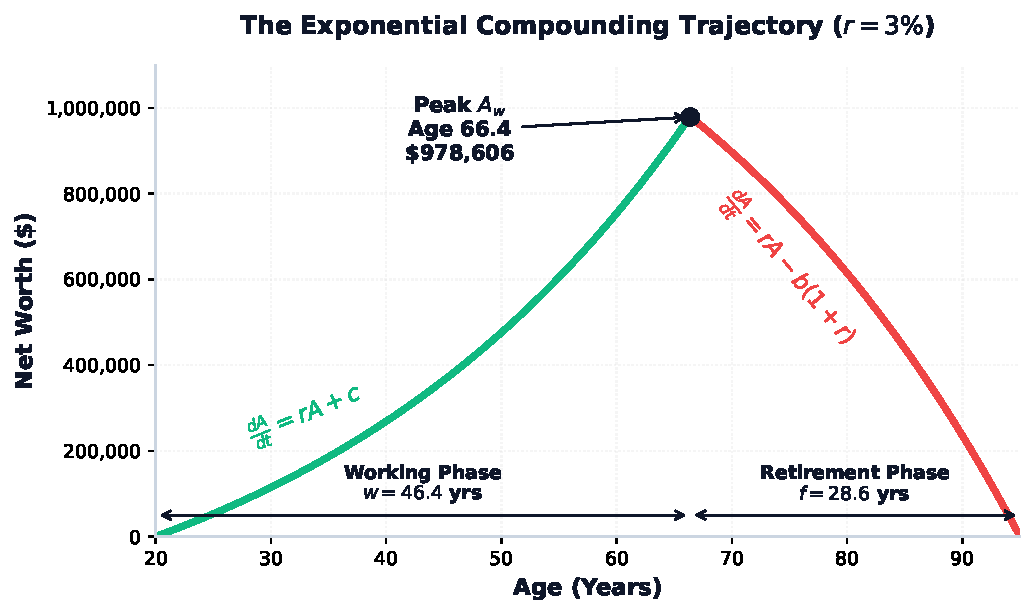
\includegraphics[width=12cm, height=6cm]{exponential_plot.pdf}
\caption{The exponential compounding lifecycle curves where $r>0\%$. The \textcolor{mpgreen}{accumulation phase} curves upward via geometric expansion and transitions to an accelerated annuity-due \textcolor{mpred}{depletion} phase.}
\label{fig:exponential_plot}
\end{figure}

% =========================================================================
% SECTION: PLOT 3 (COMPARISON TRAJECTORY)
% =========================================================================
\begin{figure}[H]
\centering
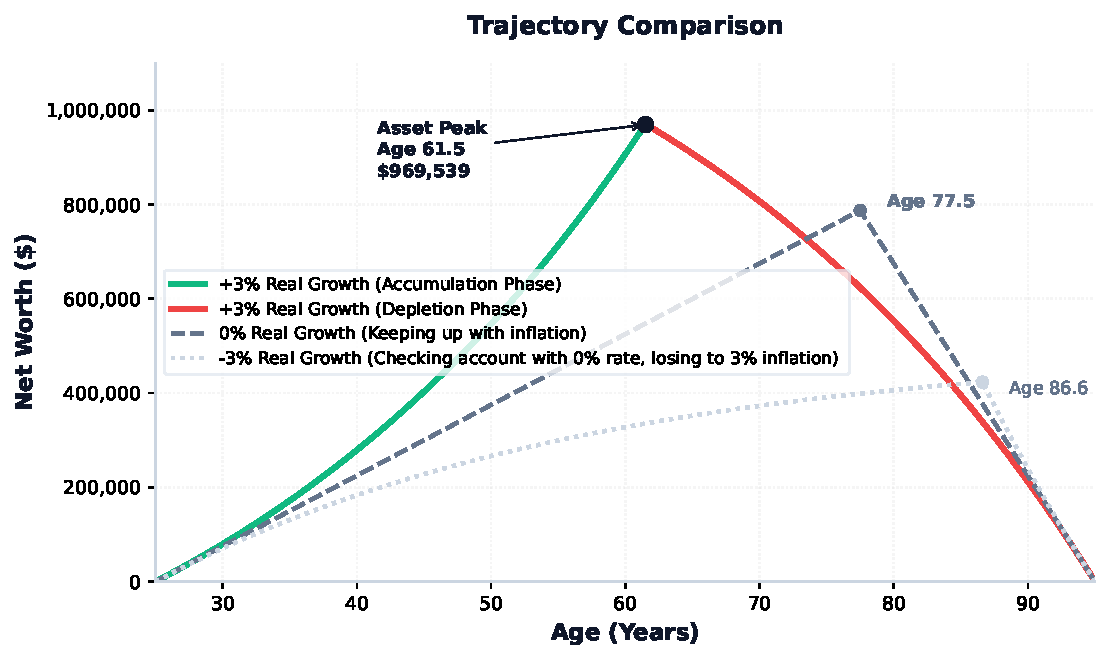
\includegraphics[width=12cm, height=6cm]{comparison_plot.pdf}
\caption{The exponential compounding curve compared to both assets just keeping with inflation and assets losing to inflation.}
\label{fig:comparison_plot}
\end{figure}

\end{document}